\section{Deelvraag 1: Stakeholders}
\label{sec:Stakeholders}
De stakeholders zijn individuen of organisaties die invloed of belang hebben bij het project.
Er is voor gekozen om de product owner als representatie te gebruiken voor de kleine bedrijven.
Dit is gedaan omdat het project nog in een proof of concept fase is en Snakeware hier nog geen klanten wil bij betrekken.
% Sommige externe stakeholders zullen gerepresenteerd worden door een gekwalificeerde interne medewerker van Snakeware.
% Dit wordt gedaan omdat de afstudeeropdracht een proof of concept is, en de klanten van Snakeware hier nog niet bij betrokken worden.
Als na de afstudeerperiode het een succes blijkt te zijn en Snakeware wil het verder ontwikkelen dan wordt contact opgezocht met de externe stakeholders (potentiële kleine bedrijven).
Er is een invloed matrix gemaakt (figuur \ref{fig:StakeholdersInvloedMatrix}) om de invloed en belang van de stakeholders te visualiseren.
Het project bestaat uit de volgende stakeholders:

\whitespace
\textbf{CEO:}
CEO Hans Hoomans is een van de oprichters van Snakeware en is verantwoordelijk (samen met de andere directieleden) voor de toekomstvisie van Snakeware.
Tijdens het opstellen van de opdracht is al aangegeven dat Hans veel ideeën heeft voor een nieuw \gls{CMS} als een product onder Snakeware.
Hierom is besloten om hem mee te nemen in het project om de toekomstvisie te integreren in het project.

\whitespace
\textbf{Product Owner:}
De product owner Elsa Croes is een projectmanager van de huidige kleine bedrijven die Snakeware heeft.
Samen met de product owner wordt de progressie bijgehouden van het project, en tijdens de realisatiefase wordt de progressie gepresenteerd.
Dit wordt gedaan om te zien of het project nog op het goede pad is en mogelijk bij te sturen als de wensen van de stakeholders veranderen.

\whitespace
\textbf{Kleine bedrijven:}
De kleine bedrijven zijn de eindgebruikers van het project, hierom is het van belang om hun eisen en wensen mee te nemen in het proces.
Het project is een proof of concept hierom is ervoor gekozen om de huidige kleine klanten niet direct betrekken bij het realiseren van het systeem.
Om toch een representatie te hebben van de kleine bedrijven is er gekozen om de product owner gebruiken als gekwalificeerde medewerker om de kleine klanten te vertegenwoordigen.
De kleine bedrijven worden gebruikt als stakehoders om de gewenste functionaliteiten in beeld te brengen.

\whitespace
\textbf{Afdeling R\&D:} De afdeling R\&D van Snakeware zijn de ontwikkelaars van het huidige \gls{CMS} en kunnen veel inzicht bieden in de huidige situatie / problemen.
Tijdens de realisatie en ontwerpfase kan er advies gevraagd worden aan de backend en frontend developers van het R\&D team.
Na de afstudeerperiode wordt het project overgedragen aan het R\&D team.

\begin{graphic}
	\captionsetup{type=figure}
	\caption{Stakeholders invloed matrix}
	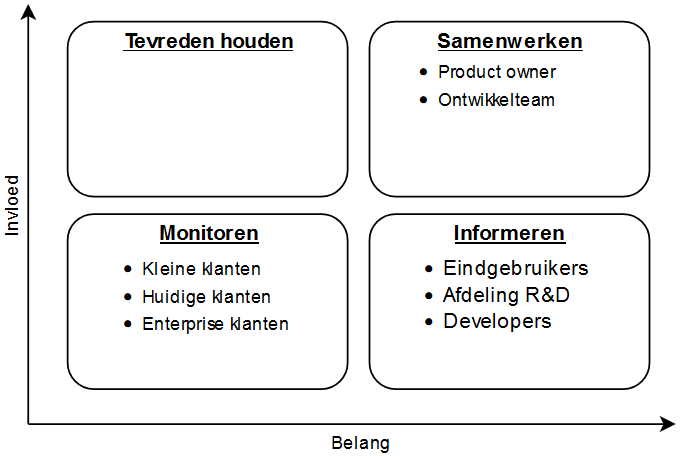
\includegraphics[scale=0.30]{StakeholdersInvloedMatrix}
	\label{fig:StakeholdersInvloedMatrix}
\end{graphic}

% \todo[inline]{Het stakeholder verhaal uitzoeken na dat de herfst vakantie (voor of kleine klanten er we of niet er tussen moeten staan).}
% \todo[inline]{De afbeelding klopt niet omdat hans er nog niet tussen staat en van wege het verhaal hier boven ik pas deze afbeelding aan als er bekend is wat er moet gebeuren met het verhaal hier boven.}
% \todo[inline]{Net zoals ik zei in methodologie, als ik de product owner ben zou elsa dan de representatie zijn voor de kleine klant? Dit is vaag }
% \todo[inline]{Als er woorden over zijn maak een kleine samenvatting voor het resultaat}
